\chapter{Differenz Pipeline}
\label{diffPipe}

Die folgenden Abschnitte dokumentieren die Implementierung des in \cite{KeKT2011ASE} beschriebenen
Konzepts des Semantic-Liftings. Die einzelnen Teile des Konzepts werden dabei in Bezug auf
ihre technische Umsetzung nochmal im Detail untersucht. Es wird dabei auch auf aufgetretene Probleme
und ggf. auf deren Lösungsansatz eingegangen.

\begin{figure}[htbp]
  \centering
  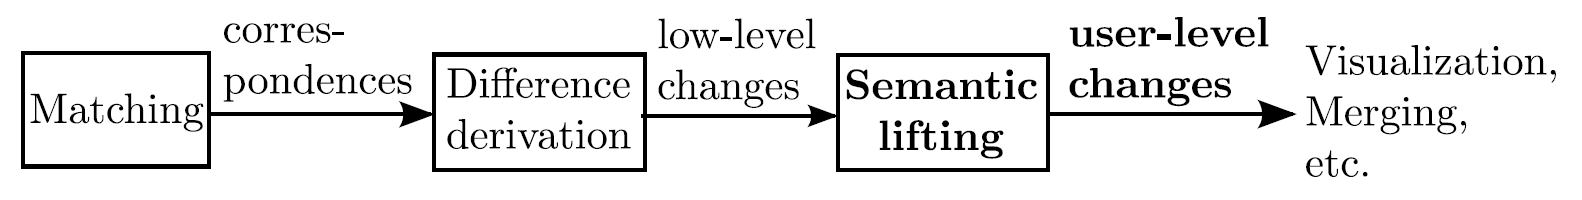
\includegraphics[scale=0.2]{images/difference_pipeline.png}
  \caption{Differenz Pipeline \cite{KeKT2011ASE}}
  \label{fig:diff_pipeline}
\end{figure}

Die Architektur des Semantic-Lifting Algorithmus lässt sich als Pipeline beschreiben, wie in
Abbildung \ref{fig:diff_pipeline} dargestellt. Als Eingabe für diese Pipeline dienen immer zwei
Versionen eines Modells. Diese beiden Versionen werden im Folgenden immer als \textbf{Modell A} und
\textbf{Modell B} bezeichnet, wobei Modell A  als die Ausgangsversion des Modells betrachtet wird,
während Modell B eine spätere Version des Modells darstellt, in der im Vergleich zu Modell A
verschiedene Teile hinzugefügt oder entfernt wurden. Als technische Grundlage für die
Implementierung dient das Eclipse Modeling Framework (EMF). Daher können nur Modelle verglichen
werden, die auf dem EMF eigenen Metamodell Ecore basieren. Im Rahmen dieses Proof-Of-Concepts
verwenden wir Ecore direkt als Metamodell für die zu vergleichenden Modelle. Grundsätzlich können
aber auch z.B. auf Ecore basierende UML Klassendiagramme oder Zustandsautomaten als Eingabe dienen,
wie Abbildung \ref{fig:metaebenen} illustriert. In allen Fällen bildet Ecore einen
selbstreferentiellen Abschluss der Abstraktionsebenen als Meta-Metamodell.

\begin{figure}[htbp]
  \centering
  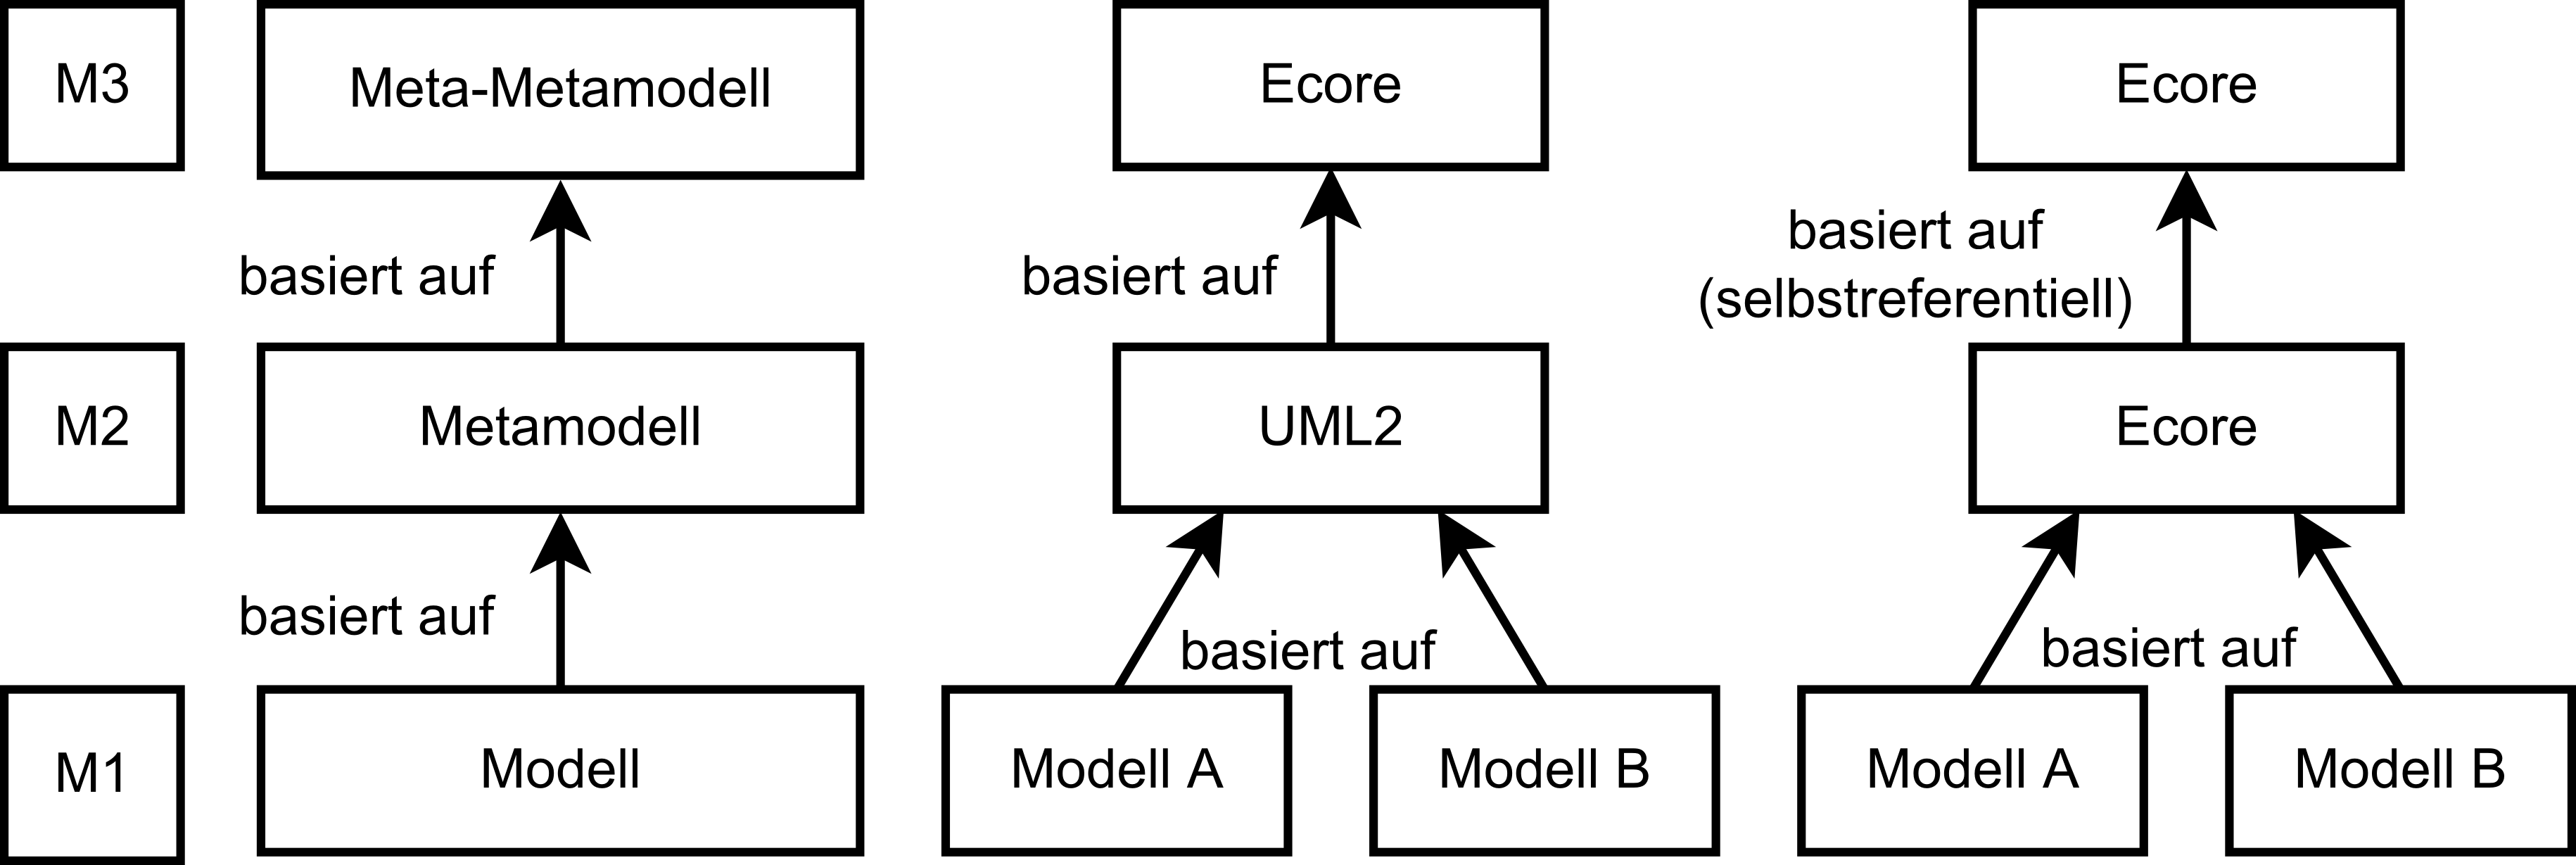
\includegraphics[width=1.0\textwidth]{images/metaebenen.png}
  \caption{Metaebenen}
  \label{fig:metaebenen}
\end{figure}

Die Modelle A und B werden dann in den folgenden Schritten weiter verarbeitet. Der erste Schritt auf
dem Weg zur semantisch gelifteten Differenz ist das Matching (Abschnitt \ref{sec:matching}). In
dieser Phase wird versucht den Elementen aus Modell A die entsprechend gleichen Element aus Modell B
zuzuordnen. Den nächsten Schritt bildet die Differenz-Ableitung (Abschnitt
\ref{sec:diff:derivation}), in der die später zu verarbeitende technische Differenz aus den
Matchings erzeugt wird. Im letzten Schritt erfolgt das Semantic-Lifting (Abschnitt
\ref{sec:lifting}), hier wird aus der technischen Differenz eine semantisch geliftete Differenz
berechnet.

% Matching
\section{Matching}
\label{sec:matching}

Als Matching wird in diesem Zusammenhang der Prozess bezeichnet, in dem die beiden Modelle A und B
miteinander verglichen werden. Dazu werden zustandsbasierte Vergleichsalgorithmen verwendet, welche
eine symmetrische Differenz auf der Basis des aktuellen Zustands der beiden Modelle berechnen.  Ziel
des Matchings ist es herauszufinden welche Elemente in beiden Modellen übereinstimmen. Diese
Übereinstimmungen werden als Korrespondenzen (\textit{engl. Correspondence}) zwischen Modellen A und
B bezeichnet. \cite{KeKT2011ASE} (S.3)

\begin{quote}
\centering
$A \Delta B := \{x \mid (((x \in  A)\wedge(x \not\in B))\vee((x \in B)\wedge(x \not\in A))) \}$
\end{quote}

\begin{figure}[htb]
  \centering
  \includegraphics[scale=0.4]{images/symmetrische_Differenz.png}
  \caption{Symmetrische Differenz}
  \label{fig:sym_diff}
\end{figure}

Die Korrespondenzen geben zunächst die Schnittmenge zwischen den Modellen an. Für die Berechnung der
korrespondierenden Elemente gibt es grundsätzlich verschiedene (zustandsbasierte) Techniken und
Algorithmen:

\begin{itemize}
  \item \textbf{ID-basiert:} In diesem Ansatz wird davon ausgegangen, dass jedes Modell-Element eine
  eindeutige statische ID besitzt. D.h. diese ID wird beim Erzeugen des Elements vergeben und darf
  sich auch im weiteren Entwicklungsverlauf des Modells nicht verändern. Der Hauptvorteil dieses
  Ansatzes besteht darin, dass keine spezielle Konfiguration für unterschiedliche Modelltypen nötig
  ist. Außerdem lassen sich Korrespondenzen sehr effizient berechnen. Dieser Ansatz funktioniert
  allerdings nicht für Modelle, die unabhängig voneinander erzeugt wurden. Außerdem muss die Vergabe
  von IDs durch die verschiedenen Entwicklungsumgebungen gewährleistet sein. \cite{KPRP2009} (S.2)
  
  \item \textbf{Signaturbasiert:} In diesem Ansatz wird eine Signatur zum vergleichen der
  Modell-Elemente verwendet. Im Gegensatz zu einer ID ist die Signatur nicht statisch. Eine Signatur
  wird dynamisch aus den Werten der Eigenschaften eines Elements berechnet. Daher können auf diese
  Weise auch Modelle verglichen werden, die unabhängig voneinander entwickelt wurden. Dieser
  Ansatz ist allerdings mit deutlich mehr Aufwand verbunden, da für jeden Modell-Element-Typ eine
  Berechnungsfunktion für die jeweilige Signatur angelegt werden muss. \cite{KPRP2009} (S.3)
  
  \item \textbf{Ähnlichkeitsbasiert:} In diesem Ansatz werden Modelle als typisierte, attributierte
  Graphen behandelt. Die einzelnen Modell-Elemente werden dabei durch die Summe ihrer Eigenschaften
  identifiziert. Dabei sind nicht alle Eigenschaften gleich wichtig. Hierzu wird in den meisten
  Algorithmen eine Konfiguration benötigt die das relative Gewicht der einzelnen Eigenschaften
  angibt. Herauszufinden welche Gewichtung der Eigenschaften für eine Modellierungssprache ein
  möglichst optimales Ergebnis liefert, ist allerdings häufig ein "`trial-and-error"' Prozess.
  Außerdem können generische Ansätze keine Rücksicht auf die Semantik der Modellierungssprache
  nehmen, welche die Genauigkeit verbessern und die Anzahl der individuellen Vergleiche verringern
  würde. \cite{KPRP2009} (S.3)
  
  \item \textbf{Sprachspezifisch:} Ein sprachspezifischer Matching Algorithmus wurde speziell für
  eine Modellierungssprache implementiert. Da diese Algorithmen die Semantik ihrer
  Modellierungsprache kennen ist hier in der Regel auch kein Semantic-Lifting notwendig. Daher wird
  hier auch nicht näher auf solche Algorithmen eingegangen. Der Nachteil dieses Ansatzes bestehen
  im hohen Entwicklungsaufwand und der auf die Modellierungssprache eingeschränkten Benutzbarkeit.
\end{itemize}
Zur Berechnung der Korrespondenzen für das Semantic-Lifting kann grundsätzlich ein beliebiger
Algorithmus verwendet werden. Die Korrespondenzen müssen nur immer in die interne Darstellung
konvertiert werden. (Siehe \texttt{Correspondeces} Abbildung \ref{fig:diffmodel}.) Ein Vergleich
verschiedener Ansätze ist in \cite{KPRP2009} zu finden. Im folgenden wird nun auf die im Rahmen
dieser Arbeit verwendeten Algorithmen eingegangen.

% Beim Vergleichen von Modellen spielt immer auch die Struktur eine wichtige Rolle. In Ecore werden
% Modelle in Form einer Baumartigen Aggregationsstruktur aufgebaut. Die einzelnen Elemente dieser
% Struktur sind typisiert und ggf. attributiert. Dabei können Elemente dieser Struktur hinzugefügt
% oder entfernt werden. Im Sinne einer Struktur kann man auch von Verschiebung einzelner Elemente
% sprechen, wenn ein Element aus einem Teilbaum einem anderen zugeordnet wird. Die Verschiebung äußert
% sich in einem Modell durch das verändern der Referenzen zwischen Container und Element. Ist das
% Element kein Blatt in der Baumstruktur so können auf diese Weise auch ganze Teilbäume verschoben
% werden. In vielen Fällen kann es wünschenswert sein ein Verschieben als solches zu erkennen und
% nicht als löschen und einfügen von Elementen. In diesem Fall würden dann Korrespondenzen zwischen
% den Verschobenen Elementen bzw. Teilbäumen angelegt, nicht aber zwischen den veränderten Referenzen
% der Container und  der Elemente bzw. Wurzeln der Teilbäume. Korrespondenzen können außerdem
% zwischen nicht gleichen Elementen auftreten. Zum Beispiel kann ein Element auf Grund seiner
% strukturellen Anordnung als Korrespondierend angesehen werden, möglicherweise wurden aber Attribute
% wie der Name des Elements verändert. Auf Grund dieser verschiedenen Eigenschaften muss
% die Menge der Korrespondenzen je nach verwendetem Matching Algorithmus nicht immer Eindeutig sein.

\subsection{SiDiff}
\label{sidiff}

SiDiff ist ein an der Universität-Siegen entwickelter Metamodell unabhängiger Ansatz, um Modelle zu
vergleichen. Der Algorithmus ist hauptsächlich darauf ausgelegt Modell-Elemente nach ihrer
Ähnlichkeit zu vergleichen (ähnlichkeitsbasiert), unterstützt aber auch Ansätze zum ID-basierten
oder signaturbasierten Modellvergleich. Der Hauptvorteil von SiDiff besteht darin, dass dem
Benutzer eine sehr frei konfigurierbare Umgebung geboten wird, die auf jeden Modelltyp angepasst
werden kann. Der Modelltyp muss sich lediglich als graphähnliche Struktur darstellen lassen. Der
generische Algorithmus muss für jeden Modelltyp konfiguriert werden. Eine Konfiguration besteht aus
einer Transformation vom Originaldokument in die interne Repräsentation, einer Definition für die
Gewichtung der Eigenschaften der zu vergleichenden Modell-Elemente für die Berechnung der
Ähnlichkeiten und einer Spezifizierung der auszugebenden Daten. \cite{SiDiff}

% SiDiff is an meta model-independent approach to model comparison. It is primarily based on the
% notion of similarity between model elements, but covers other approaches like id-based or
% signature-based model comparison as well. The main advantage of SiDiff is that it offers a highly
% configurable environment and is therefore easily adaptable to any model type where models can be
% represented in a graph-like structure
% 
% The generic algorithm must be configured for each type of model. A configuration consists of a
% transformations from the original document into an internal structure, the definition of the
% similarity of elements, a specification of the output, and further details.

\subsection{Named-Element-Matcher}
\label{nem}

Der Named-Element-Matcher wurde im Rahmen diese Projekts als Testwerkzeug verwendet, er vergleicht
die beiden Modelle A und B einfach anhand der Namen der einzelnen Elemente. Der Matcher eignet sich
vor allem für selbst konstruierte Testfälle, da das Ergebnis des matchings relativ gut abzusehen
ist. Dieser Algorithmus lässt sich als ein signaturbasierter Algorithmus einordnen. Als Signatur
wird in diesem Fall eben nur der Namen benutzt.


% Differenz-Ableitung
\section{Differenz-Ableitung}
\label{sec:diff:derivation}

Die Differenz-Ableitung ist der zweite Schritt zur Berechnung einer symmetrischen Differenz zwischen
Modell A und B. In diesem Schritt werden die Objekte identifiziert, die nicht in der Schnittmenge
der beiden Modell sind. Die so berechnete Differenz wird im Folgenden als \textbf{technische
Differenz} bezeichnet. Eine technische Differenz teilt sich zunächst in zwei Klassen ein:
\texttt{Correspondence} und \texttt{Change}. Die zuvor im Matching berechneten Korrespondenzen der
Schnittmenge werden durch Objekte der Klasse \texttt{Correspondence} dargestellt. Die Summe aller
\texttt{Correspondence} gibt damit die gemeinsamen Teile von Modell A und Modell B an. Die Teile,
die sich von Modell A zu Modell B unterscheiden, werden durch Objekte der Klasse \texttt{Change}
(Änderung) angegeben. Bei Änderungen an einem Modell unterscheiden wir dabei noch zusätzlich
zwischen den drei Grundelementen eines Modells: Objekte, Referenzen und Attribute. Objekte und
Referenzen können in ein Modell sowohl eingefügt als auch entfernt werden. Ausgehen davon, dass wir
keine mehrwertigen Attribute betrachten, sind hingegen einwertige Attribute durch die Metaklassen
fest vorgegeben und können daher nur einen neuen Wert zugewiesen bekommen. Zu diesem Zweck werden
folgende Klassen definiert:

\begin{itemize}
  \item \texttt{Add-Object}: In Modell B existiert ein Objekt, welches nicht in Modell A existiert.
  Das Objekt wurde also in Modell B hinzugefügt.
  
  \item \texttt{Remove-Object}: In Modell A existiert ein Objekt, welches nicht in Modell B
  existiert. Das Objekt wurde also in Modell B entfernt.
  
  \item \texttt{Add-Reference}: In Modell B existiert eine Referenz, welche nicht in Modell A
  existiert. Die Referenz wurde also in Modell B hinzugefügt.
  
  \item \texttt{Remove-Refernce}: In Modell A existiert eine Referenz, welche nicht in Modell B
  existiert. Die Referenz wurde also in Modell B entfernt.
  
  \item \texttt{Attribute-Value-Change}: Für alle Objekte aus Modell A und Modell B, für die eine
  Korrespondenz existiert, wird überprüft, ob sich der Wert eines Attributs verändert hat und ggf.
  ein Attribute-Value-Change erzeugt. Es werden keine Attribute-Value-Changes für neue
  initialisierte Attribute eines Add-Objects angelegt.
  
  Attribute, deren Metatyp (\texttt{EAttribute}) folgende Eigenschaften haben, können dabei
  vernachlässigt werden, da sich aus diesen Attributen keine direkten Änderungen des Modells
  ableiten lassen:
  
  \begin{itemize}
    \item\texttt{changeable = false} $\to$ Der Wert kann von außen nicht verändert werden. D.h. es
    wird keine \texttt{setXX()} Methode generiert. \cite{SBPM2009} (S. 108)
    
    \item\texttt{transient = true} $\to$  Der Wert wird bei der Serialisierung übergangen und nicht
    mit abgespeichert. \cite{SBPM2009} (S. 108)
    
    \item \texttt{derived = true} $\to$ Gibt an, dass dieser Wert aus anderen Informationen
    abgeleitet wird. Hat aber keinen Einfluss auf die Code Generierung. \cite{SBPM2009} (S. 108)
  \end{itemize}
\end{itemize}
Das in Ecore Implementierte Differenzmodell ist in Abbildung \ref{fig:diffmodel} zu sehen. Es bildet
die Basis für das spätere Semantic-Lifting. Die in dieser Phase berechneten \texttt{Changes} werden
im Folgenden als \textbf{low-level Änderungen} bezeichnet, da die durchgeführten Änderungen am
Modell hier noch auf einer rein technischen Ebene angegeben werden.

\begin{figure}[htb]
  \centering
  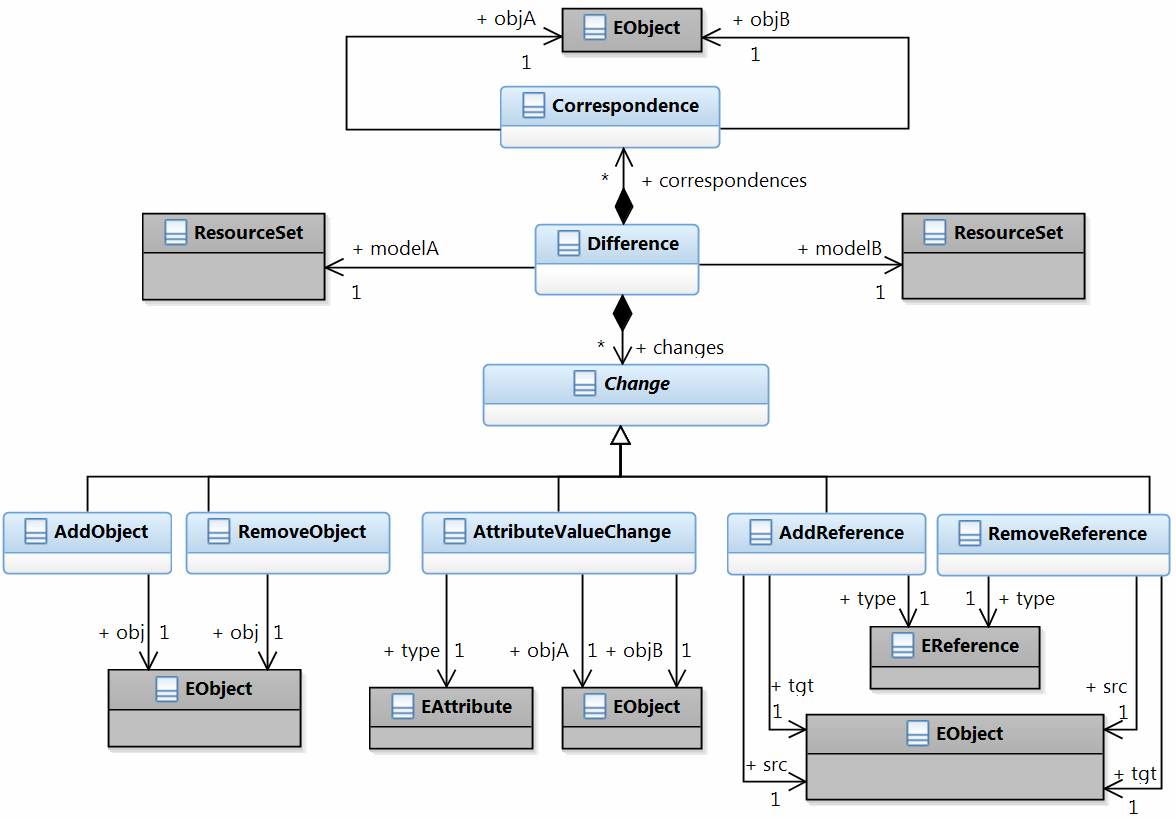
\includegraphics[width=1.0\textwidth]{images/difference_model.png}
  \caption{Differenzmodell}
  \label{fig:diffmodel}
\end{figure}

% Semantic-Lifiting
\section{Semantic-Lifting}
\label{sec:lifting}

Als Eingabe für das Semantic-Lifting dient die zuvor berechnete technische Differenz der Modelle A
und B. Die technische Differenz enthält ausschließlich low-level Änderungen, welche angeben, was
sich zwischen Modell A und Modell B verändert hat. Da low-level Änderungen auf Basis des Metamodells
angegeben werden, sind diese aber für normale Benutzer oft sehr unverständlich. Auch um einen
schnellen Überblick über die Veränderungen eines Modells zu bekommen, eignet sich diese Form der
Repräsentation nicht besonders gut, da die low-level Änderungen unstrukturiert in der Differenz
liegen. Aus Benutzersicht wäre es wünschenswert die low-level Änderungen so zu strukturieren, dass
sie den Bearbeitungsprozess eines Editors wiedergeben. Genau dieses Ziel verfolgt das
Semantic-Lifting, die technischen Änderungen wieder als Editieroperation auf einer Benutzer
verständlichen Ebene darzustellen. 

Um eine Editieroperation darzustellen, werden die low-level Änderungen neu strukturiert. Jede
angewendete Editieroperation lässt sich auf ein bestimmtes Muster in der Differenz zurückführen.
Dieses Muster besteht sowohl aus low-level Änderungen als auch aus einem bestimmten Kontext. Der
Kontext einer Editieroperation gibt zum einen an, auf welche Elemente die Editieroperation
angewendet werden soll, zum andern können bestimmte Umstände vorgegeben sein, damit der Vorgang
ausgeführt werden darf. Welche Änderungen in welchem Kontext von einer Editieroperation ausgeführt werden, wird
durch die s.g. \textbf{Editierregel} vorgegeben. Aus dieser Editierregel kann dann das Muster
abgeleitet werden, das die Editieroperation in einer Differenz wieder erkennt. Dieses Muster wird
als \textbf{Erkennungsregel} bezeichnet. Das Muster einer Erkennungsregel überprüft die Differenz sowohl
auf auftretende low-level Änderungen als auch auf den Kontext der entsprechenden Editieroperation.
Nachdem also eine bestimmte Editieroperation in der Differenz erkannt wurde, können die
entsprechenden low-level Änderungen der Editeroperation wieder zugeordnet werden. Um diese
semantische Zuordnung von Editieropration zu low-level Änderungen in der Differenz zu speichern,
wird eine neu Klasse in unser Differenzmodell eingeführt. Wie in Abbildung \ref{fig:scs} zu sehen
ist, gruppiert ein s.g. \textbf{Semantic-Change-Set} mehrere zu einer Editieroperation gehörenden
low-level Änderungen (\texttt{Change}). Der Name des Semantic-Change-Sets entspricht der
assoziierten Editieroperation. Dabei ist darauf zu achten, dass am Ende des Semantic-Lifitngs jede
low-level Änderung nur in einem Semantic-Change-Set enthalten ist. Im Semantic-Lifting Konzept  wird
dies wie folgt formuliert:
\begin{quote}
"`The objective of semantically lifting a model difference is thus to partition the set of low-level
changes into disjoint subsets, each subset containing the changes belonging to exactly one edit
operation. These subsets must be disjoint since each low-level change results from the application
of exactly one edit operation. We call these subsets \textbf{semantic change sets}."'
\cite{KeKT2011ASE} (S.5)
\end{quote}

\begin{figure}[htb]
  \centering
  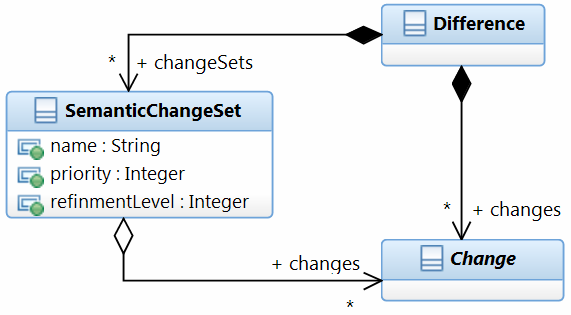
\includegraphics[scale=0.5]{images/semantic_change_set.png}
  \caption{Semantic-Change-Set}
  \label{fig:scs}
\end{figure}